\documentclass[12pt]{article}

%%%%%%% PACKAGES %%%%%%%%
\usepackage[utf8]{inputenc}
\usepackage[margin=2.3 cm]{geometry}
\usepackage{blindtext}
\usepackage{graphicx}
\usepackage{notoccite} %citation number ordering
\usepackage{lscape} %landscape table
\usepackage{caption} %add a newline in the table caption
\usepackage{float} %Package for using the [H] option on graphics to force them into place
\usepackage{enumerate} % Needed for markdown enumerations to work
\usepackage{url}
\usepackage[hidelinks]{hyperref}
\usepackage[nohyperlinks]{acronym}
\usepackage{graphicx}
\usepackage{fancyhdr}
\usepackage[]{xcolor}
\usepackage{footnote}
\usepackage{tikz}
\usepackage{pgfplots}
\usepackage{todonotes}
\usepackage{titlesec}

\setlength{\parindent}{0pt} % no indent at paragraph start

\usepackage[
backend=biber,  %references format (IEEE)
style=ieee,
sorting=none
]{biblatex}
\addbibresource{refs.bib} %rename this to your own bibliography

\titlespacing*{\section} {0pt}{2 ex}{1ex}
\titlespacing*{\subsection} {0pt}{2 ex}{1ex}
\titlespacing*{\subsubsection} {0pt}{2 ex}{1ex}

\titleformat*{\section}{\large\bfseries}
\titleformat*{\subsection}{\normalsize\bfseries}
\titleformat*{\subsubsection}{\normalsize\bfseries}

\title{\huge{\textbf{STA302 Final Report}} \\
\LARGE{Between speed, spin, movement, release point, extension, and command, which (if any) affected the whiff percent on a four seam fastball in 2023?}}
\author{Grace Shang}
\date{17 June 2024}

\renewcommand\floatpagefraction{.9}
\renewcommand\topfraction{.9}
\renewcommand\bottomfraction{.9}
\renewcommand\textfraction{.1}   
\setcounter{totalnumber}{50}
\setcounter{topnumber}{50}
\setcounter{bottomnumber}{50}

\begin{document}
\pagenumbering{roman} % Start roman numbering
\clearpage\maketitle
\thispagestyle{empty}

\newpage
\setcounter{page}{1}
\tableofcontents

\newpage
\pagenumbering{arabic} % Start roman numbering

%%% CONTENT HERE %%%%
%% Intro %%
\section{Introduction}
Of the 14 officially classified pitch types in Major League Baseball, the 4-seam fastball is usually considered a pitcher's dependable, bread-and-butter choice. While not all pitchers pitch to generate swings and misses, the ability to generate whiffs is almost always considered a good one. There are so many factors involved in one pitch, however, that it is not so easy to tell what is actually causing a whiff. Using the fastball, I want to investigate some common suggestions: Its speed and spin, the amount of sideways or vertical movement, and the pitcher's extension, release point, and command. My goal will be to determine which, if any, of these factors from a pitcher can significantly contribute to predicting their whiff percent on fastballs. 

\medskip

This information should be of interest to MLB coaches and front offices. Coaches want to determine which factors to emphasize during training. Front offices want to determine if a pitcher will perform well before acquiring them. Blahill et al. (2005) discusses the effects of a pitcher's movement (release point and extension), their pitch's movement, speed, and spin on a batter's ability to detect the pitch. They do not specifically mention whiff percent or command in their analysis, however. Similarly, Selin (1959) analyzes six pitches for spin and movement, but places more of an emphasis on predicting pitch trajectory rather than whiffs. Sidhu and Caffo (2014) use ordinary least squares regression to determine pitch trajectory based on velocity and movement across different pitches, and they later use the regression in reinforcement learning to train a batter's model on pitch decision making, in part influenced by swings and misses. These papers suggest that the factors I am considering in my model are potentially significant to a pitch's performance. Note also that all three papers are at least 10 years old, and baseball analytics and pitching philosophies have changed substantially during this time, so my model will introduce a more recent insight into fastball performance. 


%% Methods %%
\section{Methods}
\subsection{Data Collection and Processing}
Data will be sourced from Baseball Savant's Statcast as well as Cameron Groove's PitchingBot on Fangraphs. Statcast provides data on a pitcher's average fastball velocity (MPH), spin (RPM, rotations per minute), downwards and sideways movement (in), release point (ft), and extension (ft). PitchingBot provides data on command (a rating of a pitcher's ability to hit target locations in different counts). To produce our working data set, we set a minimum of 500 fastballs thrown so that the averages are not products of a small sample size. Then, we combine the data provided by Statcast and PitchingBot for a total of 150 pitchers in 2023. 

\medskip

Before proceeding with modelling, we must split our data into training and validation sets. We randomly sample $80$\% of the data (120 pitchers) to put into the training set, and place the other $20$\% (30 pitchers) in the validation set. Then, we check if there are any missing or nonsensical data points that could be a result of tracking errors.

\subsection{Developing Models}
While developing our models, we follow backwards elimination. We will include all of our estimators in our first model, and then iteratively remove the least significant parameter. We will validate such decisions via partial F tests. For each model, we will check that they fit the assumptions of linear regression by reviewing observed versus fitted plots for linearity, Q-Q plots for residual normality, residual plots for homoscedasticity (correcting by variance stabilizing transformations or weighted least squares if needed), calculating VIF for multicollinearity, and identifying potential leverage points or outliers and deciding if they should be removed.

\subsection{Selecting Models}
We will use a combination of adjusted $R^2$, corrected AIC, and BIC to select the best model. We aim to maximize the first and minimize the latter two with the least amount of parameters.

\subsection{Validating Models}
Finally, we select our best performing model(s) using the criteria above and attempt to validate them by assessing their performance on the training dataset. We compare the values of parameters, the significance of each parameter, adjusted $R^2$ values, and (non)-multicollinearity. The two datasets should yield similar results. Finally, we will attempt to diagnose any issues if the model cannot be validated by comparing our training/validation data sets, searching for influential points in the validation set, and evaluating the overall quality of our model.

%% Results %%
\section{Results}
\subsection{Data Collection and Processing}
\begin{figure}[h]
    \begin{centering}
        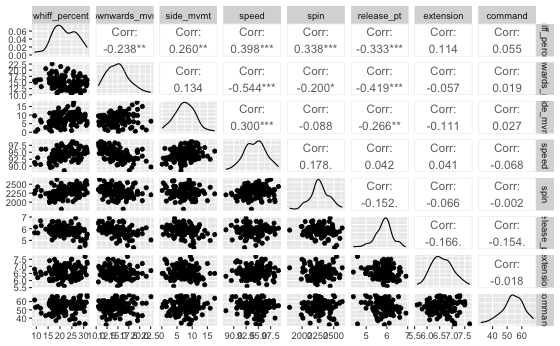
\includegraphics[scale = 0.45]{pics/corr.png}
    \caption{Correlation plot, response variable on left}
    \end{centering}
\end{figure}
Based on the figure above, most of the predictors are significantly correlated with our response variable, whiff percent. The exceptions are extension and command, although we will keep them in our initial analysis for posterity's sake. With the exception of speed versus movement and release point versus movement, the predictors appear to be uncorrelated. The range of each variable can be seen on the leftmost axis on the figure.

\medskip

It also seems like all variables are mostly linearly related with whiff percent (see the left column). With the exception of maybe command, which doesn't seem to follow any pattern at all, there does not seem to be any notable non-linear trends. There are also a few points quite far away from the rest of the data set, which we may have to deal with later.

\subsection{Developing Models}
We will use the following: $\beta_1$ for speed, $\beta_2$ for spin, $\beta_3$ for downwards movement, $\beta_4$ for sideways movement, $\beta_5$ for release point, $\beta_6$ for extension, and $\beta_7$ for command. 
\begin{center}
    \textbf{Developed Models} \\
    \begin{tabular}{|c|c|c|}
        \hline
        \textbf{Model} & \textbf{Significant Parameters} & \textbf{Partial F test} \\
        \hline
        \begin{tabular}{c}
            $y = 3.481 + 0.269x_{1i} + 0.008 x_{2i} - 0.605 x_{3i}$ \\
            $+ 0.314 x_{4i} + -4.274 x_{5i} + 0.959 x_{6i} + 0.021 x_{7i}$
        \end{tabular} & 
        \begin{tabular}{c}
            $\beta_{2}$ (**), $\beta_{3}$ (**), \\
            $\beta_4$ (*), $\beta_5$ (***)
        \end{tabular} & \\
        \hline
        \begin{tabular}{c}
            $y = 6.511 + 0.259x_{1i} + 0.007 x_{2i} - 0.616 x_{3i}$ \\
            $+ 0.315 x_{4i} + -4.361 x_{5i} + 0.933 x_{6i}$
        \end{tabular} & 
        \begin{tabular}{c}
            $\beta_{2}$ (**), $\beta_{3}$ (**), \\
            $\beta_4$ (*), $\beta_5$ (***)
        \end{tabular} & $p = 0.6586$\\
        \hline 
        \begin{tabular}{c}
            $y = 14.8399 + 0.271 x_{1i} + 0.007 x_{2i}$ \\
            $-0.641 x_{3i} + 0.289 x_{4i} -4.649 x_{5i}$
        \end{tabular} & 
        \begin{tabular}{c}
            $\beta_{2}$ (**), $\beta_{3}$ (**), \\
            $\beta_4$ (*), $\beta_5$ (***)
        \end{tabular} & $p = 0.3023$\\
        \hline
        \begin{tabular}{c}
            $y = 44.332 + 0.007 x_{2i} -0.805 x_{3i}$ \\ $+ 0.345 x_{4i} -4.984 x_{5i}$
        \end{tabular} & 
        \begin{tabular}{c}
            $\beta_{2}$ (**), $\beta_{3}$ (**), \\
            $\beta_4$ (*), $\beta_5$ (***)
        \end{tabular} & $p = 0.4534$\\
        \hline
    \end{tabular}

    \smallskip
    
    Table 1: Table including all four models developed via backwards elimination
\end{center}

\subsubsection{Model 1}
Though the first model above includes all parameters, it was not the first tested model. In the original model, point 27 (Shane Bieber) was the farthest in terms of standardized residuals at $-3.10$ (See \ref{outlier 27}). This had a negative effect on the Normal Q-Q and residual plots. Bieber exhibited an unusually low whiff percent of 9.3\% in 2023, the single lowest in our dataset, after being sidelined with elbow inflammation (a particularly impactful injury) for much of the season.  Note that no similar issue was found for other potential outliers. Since $r_{27} = -3.10$ is ``between'' boundaries of outliers, we decided given the context it would be best to remove and re-fit. This reduced residual standard error by $0.15$ and increased $R^2$ from $0.3416$ to $0.3616$. 

\medskip

Additionally, while the scale-location plot looked mostly alright (\ref{outlier 27}), there seemed to be variance concentrated in the middle. This is likely due to the response variable being a percentage, and is commonly treated using the arcsine transformation (Mordkoff, 2016). We attempted to do as such, though it did not seem to improve the issue both before and after removing our outlier (Bieber was an outlier after the arcsine transformation as well, with a worse standardized residual of $-3.4508$). Results of this transformation can be found in the appendix (\ref{asine qq}). 

\begin{figure}[h]
    \begin{centering}
        %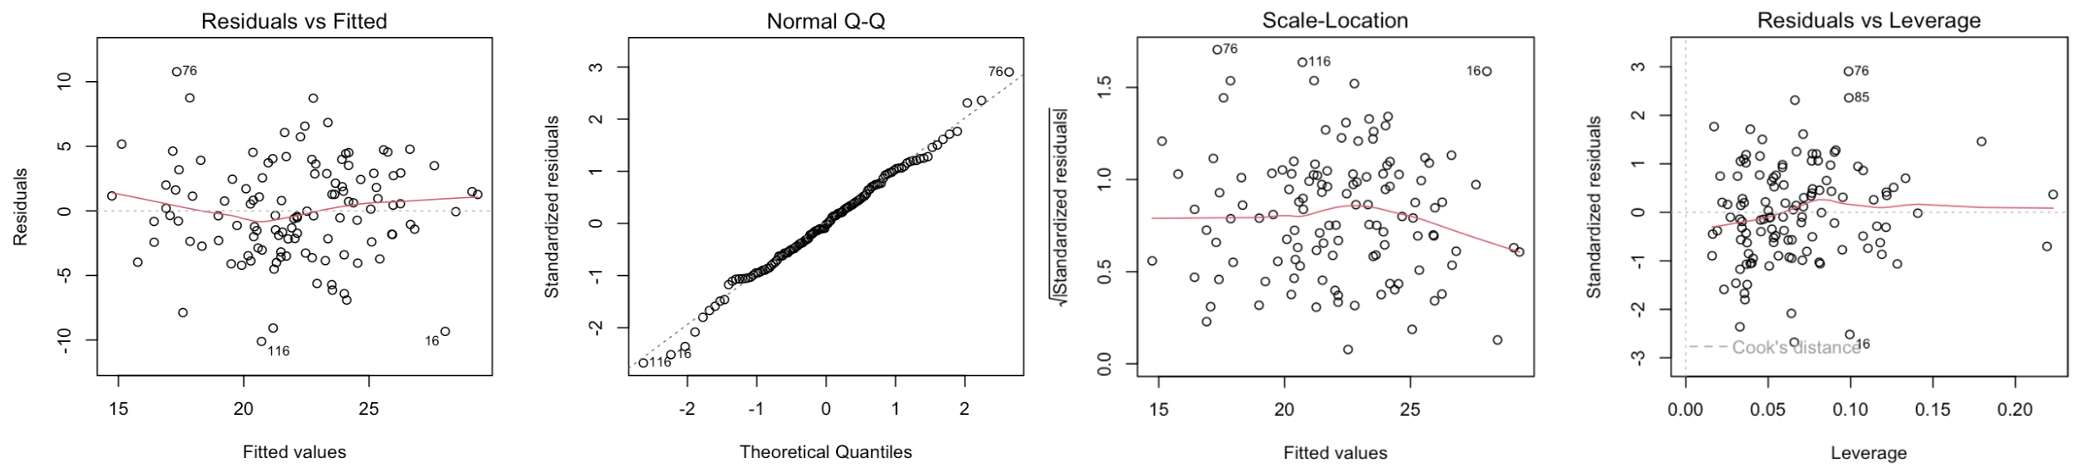
\includegraphics[scale = 0.22]{pics/model 1.jpeg}
        %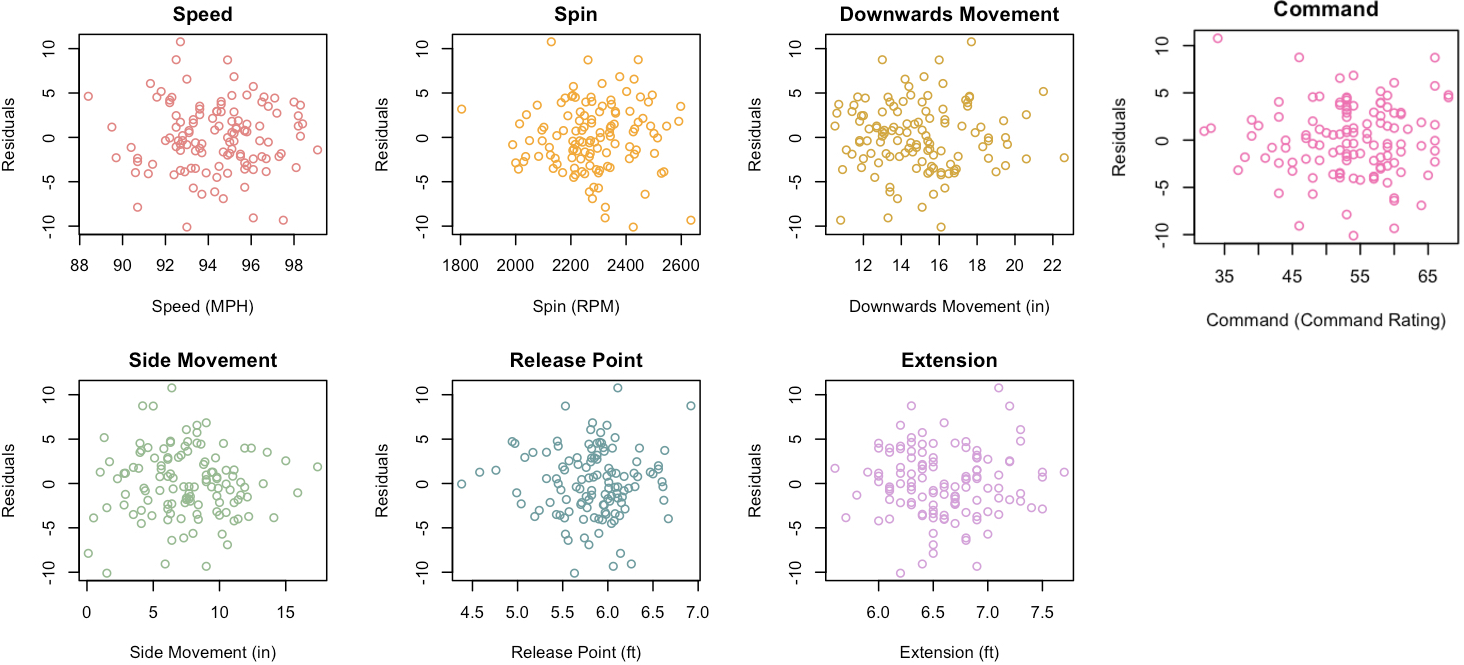
\includegraphics[scale = 0.3]{pics/model 1 plots.jpeg}
        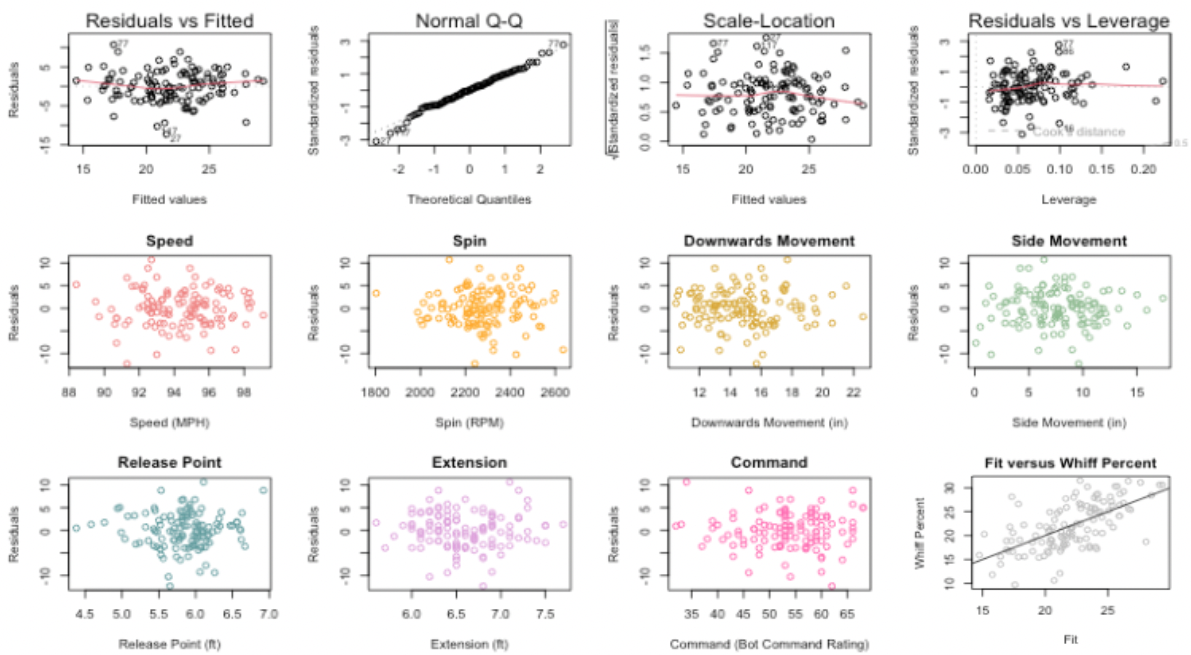
\includegraphics[scale = 0.3]{pics/mod 1 assumptions.png}
    \caption{Residual vs Fitted / Predictor, Q-Q, scale-location, leverage plots (Model 1)}
    \end{centering}
\end{figure}

Before proceeding with the model, we checked our assumptions. The simplest to address was multicollinearity: Of note were downwards movement and speed with VIFs of $2.133$ and $1.894$ respectively, though neither are larger than $5$ and so were left untreated. The plots of our first model can be found above. The removal of Bieber seemed to have improved the plots slightly. There may be a slight concern with heteroskedasticity (though it looks more like the effects of a few points instead of a pattern), but there appear to be no major violations otherwise. 

\subsubsection{Models 2, 3}
For Models 2 and 3, we removed command and extension respectively. There was no notable procedure necessary for models 2 and 3, as there were no major violations of assumptions. Partial $F$ tests indicate our procedure was valid.

\subsubsection{Model 4}
First, we removed speed. The result of our partial $F$ test indicates that all of our removals were okay. However, the heteroskedasticity issue seems to have gotten worse in the movements:
\begin{figure}[h]
    \begin{centering}
        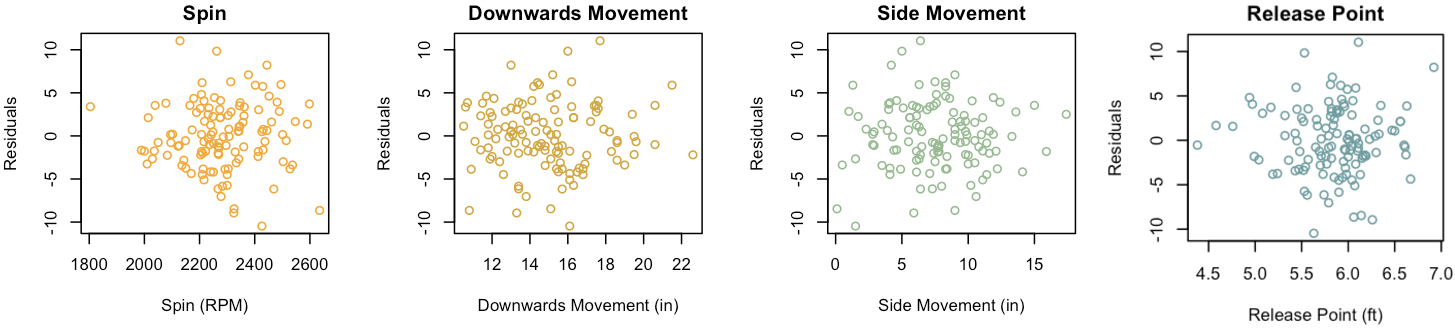
\includegraphics[scale = 0.25]{pics/heteroskedasticity.jpeg}
    \caption{Possible heteroskedasticity issues (Pre-Model 4)}
    \end{centering}
\end{figure}

\begin{figure}[h]
    \begin{centering}
        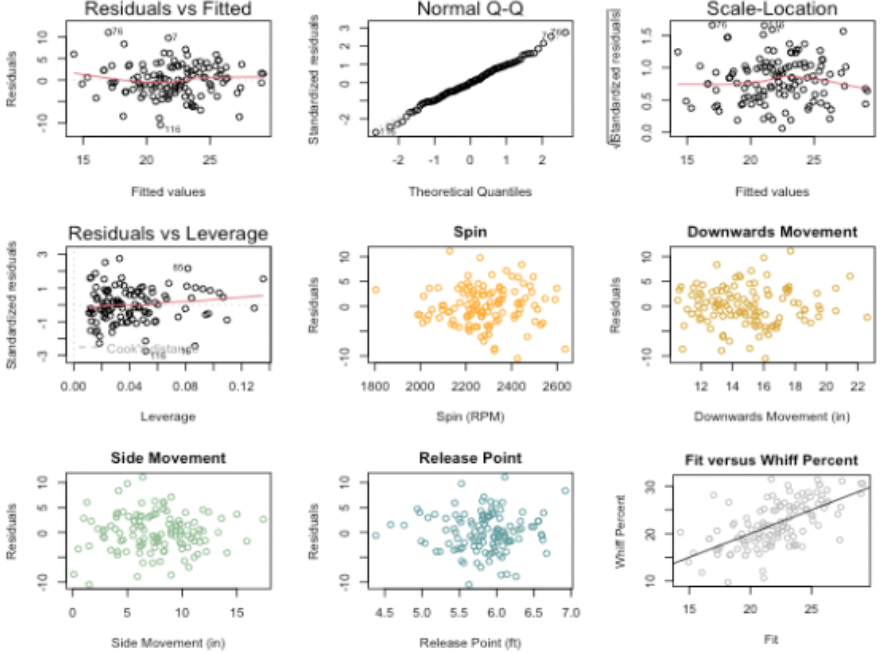
\includegraphics[scale = 0.38]{pics/mod 2 assumptions.png}
    \caption{Residual vs Fitted / Predictor, Q-Q, scale-location, leverage plots (Model 4)}
    \end{centering}
\end{figure}

We attempted to treat the concern using the arcsine transformation, but it appeared to again only have gotten worse (See \ref{asine 2}). Instead, we applied weighted least squares. The results of this can be seen in our assumption plots (Figure 4). It is a little difficult to spot visually, but the standard errors are indicative of its usefulness, decreasing residual standard error from $3.901$ to $1.292$. Additionally, VIF tells us multicollinearity remains not an issue that needs to be addressed. Attempting to remove any other parameters results in a significant partial $F$ test.

\subsection{Selecting Models}
We develop the following table (using $AICc$ since between our models, $K \geq 6$, $\frac{n}{K} \leq 19.8$).
\begin{center}
\textbf{Model Selection Table} \\
    \begin{tabular}{|c|c|c|c|c|}
        \hline
        \textbf{Model} & \textbf{Predictors} & \textbf{Adj.} $\mathbf{R^2}$ & $\mathbf{AICc}$ & $\mathbf{BIC}$ \\
        \hline
        \begin{tabular}{c}
        1
        \end{tabular} & 7 & 0.3636 & 673.4250 & 696.8155 \\
        \hline
        2 & 6 & 0.3682 & 671.2994 & 692.2466 \\
        \hline
        3 & 5 & 0.3678 & 670.1402 & 688.6030 \\
        \hline
        \begin{tabular} {c}
        4
        \end{tabular} & \textbf{4} & \textbf{0.3714} & \textbf{668.6421} & \textbf{684.5800} \\
        \hline
    \end{tabular} 

    \smallskip
    
    Table 2: Table containing model selection criteria of our four models (Best \textbf{bolded})
\end{center}

By all counts, the last model is preferable to the others. We will proceed to validation using it.

\subsection{Validating Models}
\begin{center}
\textbf{Validation Summary Table} \\
    \begin{tabular}{|c|c|c|c|c|c|c|}
        \hline
        \textbf{Dataset} & \textbf{Spin} & \textbf{Down Mvmt.} & \textbf{Side Mvmt.} & \textbf{Release Point} & \textbf{Adj.} $\mathbf{R^2}$\\
        \hline
        Training & 0.0071 (**) & -0.8052 (***) & 0.3454 (**) & -4.9842 (***) & 0.3714\\
        \hline
        Validation & 0.0055 & -1.1193 (*) & -0.1347 & -7.1247 (**) & 0.2649\\
        \hline 
    \end{tabular} \\

    \smallskip
    
    Table 3: Table summarizing training versus validation parameters and adjusted $R^2$
\end{center}

There is also no problematic multicollinearity in the testing model. Based on the table above, there seems to be signs of over-fitting, since spin and side movement are no longer significant. Spin and downwards movement are still within the standard error of training dataset, however. 

\begin{figure}[h]
    \begin{centering}
        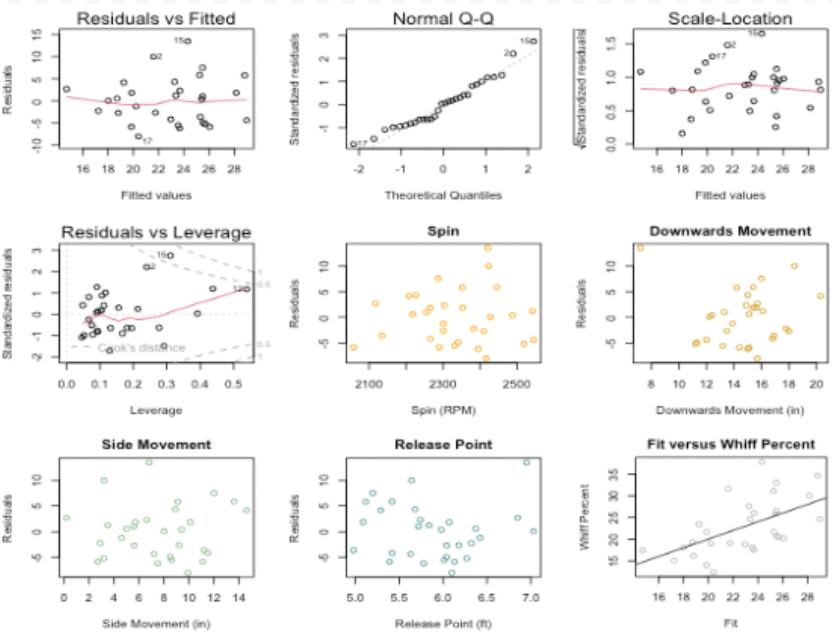
\includegraphics[scale = 0.33]{pics/val assumptions.png}
    \caption{Residual vs Fitted / Predictor, Q-Q, scale-location, leverage plots (Validation)}
    \end{centering}
\end{figure}

A look at the plots tells us there is no major issue in assumptions besides maybe normality and heteroskedasticity (More details about the above diagrams will be discussed in the next section). However, due to the difference in $R^2$, it is hard to say the model has been validated. 


% Results section: where you present a numerical/graphical description of your study sample and important results that led you to make crucial decisions in building your model (following the methods you outline in the earlier section), followed by the final model and any other important results.

% When presenting your results, avoid repeating exactly what you wrote in your methods section. Instead, focus on the results of the process you described earlier, and use numerical values/graphical results to support the decisions you made in arriving at your final model.

%% Discussion
\section{Discussion}
Our goal throughout this project was to determine which, if any, of the tested parameters had an effect on a fastball's ability to generate whiffs. Based on our selected model, a fastball's spin, downwards movement, sideways movement, and release point are the most influential factors in determining it's whiff rate. Per the model, increasing spin and sideways movement positively affect a pitcher's fastball whiff percent, whereas decreasing drop (giving the illusion of a ``rising fastball") and the release point increase whiff percent on fastballs the most. For instance, for every additional inch of release point on a fastball, the whiff percent decreases around $ 4.98 \pm 0.98$\% ($0.98\%$ being the standard error of the coefficient), so it generally seems preferable to release as low as possible.

\medskip

It should be noted that the final adjusted $R^2$ in both datasets is not spectacular: In the training data, it only explained about 37\% of the variation in the data, and in the validation data, it performed even worse at about only 26\% of the variation. After further consideration, this seems reasonable; After all, the outcome of a pitch depends not only on the pitcher, but also on the person hitting the pitch. For instance, the four teams in the NL West division except for Colorado were all in the top third at making contact with fastballs in 2023. Aside from Houston, the other four teams in the AL West division were the opposite; They were composed of some of the worst teams at making contact. Since teams face opposing teams in their division more often, pitchers from Colorado and Houston may be hurt or helped respectively. Peter Lambert (Colorado) and Hector Neris (Houston) are examples; Their numbers in the chosen parameters are actually very similar, yet the former had a whiff percent of 16.7\% and the latter had a whiff percent of 29.0\% (though worth noting 2023 was Neris' best career year). Our model indeed over-estimates Lambert's actual posted whiff percent by 3.8\% and under-estimates Neris's by 5.8\%. To adjust for this, it is theoretically possible to add indicators that correspond to the teams they face most often; However, this would require an additional 29 parameters to track and is not practical for this project. 

\medskip

As noted previously, there are concerns about the validity of the model due to possible over/under-fitting. It is also worth looking into the testing data itself, however. From Figure 5, we can see that there is certainly one  point (5, Felix Bautista, posting the highest whiff percent in the dataset) that raises concern for influence, and two points that are close (2, 12). Since these are in the validation set, however, we cannot remove them. Further investigation into the summary statistics provides a possible explanation for this difference: The whiff percent in the validation data has almost double the variance ($41.3285$) of the training data ($23.9954$). The average number of fastballs thrown by pitchers in the training data ($1981.277$) was almost 100 more than that of the validation data ($1884.667$), which might explain some of the variance. Again, however, these issues cannot be resolved since we cannot re-train our model based on the validation data. Future study into this material might warrant looking at a larger sum of data across different years, though a good selection of seasons may be difficult since the game has rapidly changed over the last fifteen or so years due to the introduction of new rules and rapidly improving players and analytics. 

% Discussion section: where you interpret your final model and describe why it answers
% the research question and why it is important, as well as discuss any limitations that
% still exist based on your results.

% You may use tables and plots to help present your results, but they must be relevant and well thought-out to convey as much information as possible without being too overwhelming or confusing. 

% An interpretation (in
% context and correct)
% is provided for at
% least one coefficient
% in the final model
% AND a general
% summary of what the
% model tells us
% about the
% relationship between
% predictors and
% response is provided
% AND it is emphasized
% how the final model
% answers the research
% question.


% All lingering
% problems with the
% final model are
% correctly mentioned
% AND their potential
% impact on usefulness
% of final model
% correctly discussed
% AND a correct
% justification is
% provided for
% why/how they could
% not be corrected.

\newpage

%% Appendix
\section{Appendix}

\center{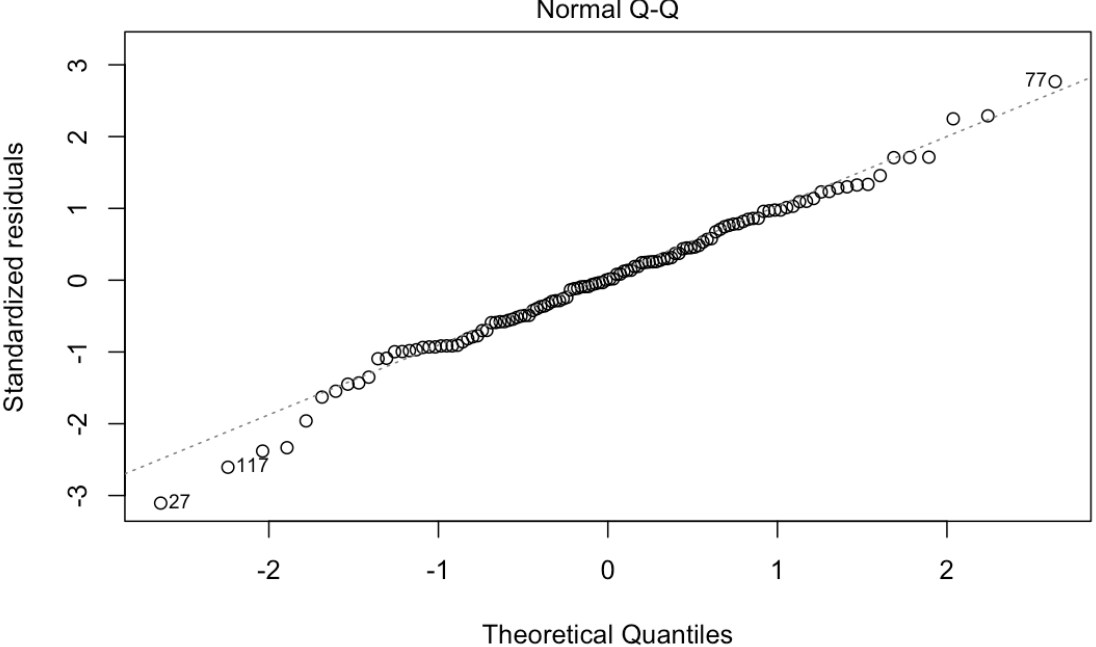
\includegraphics[scale = 0.4]{pics/outlier qq.png} 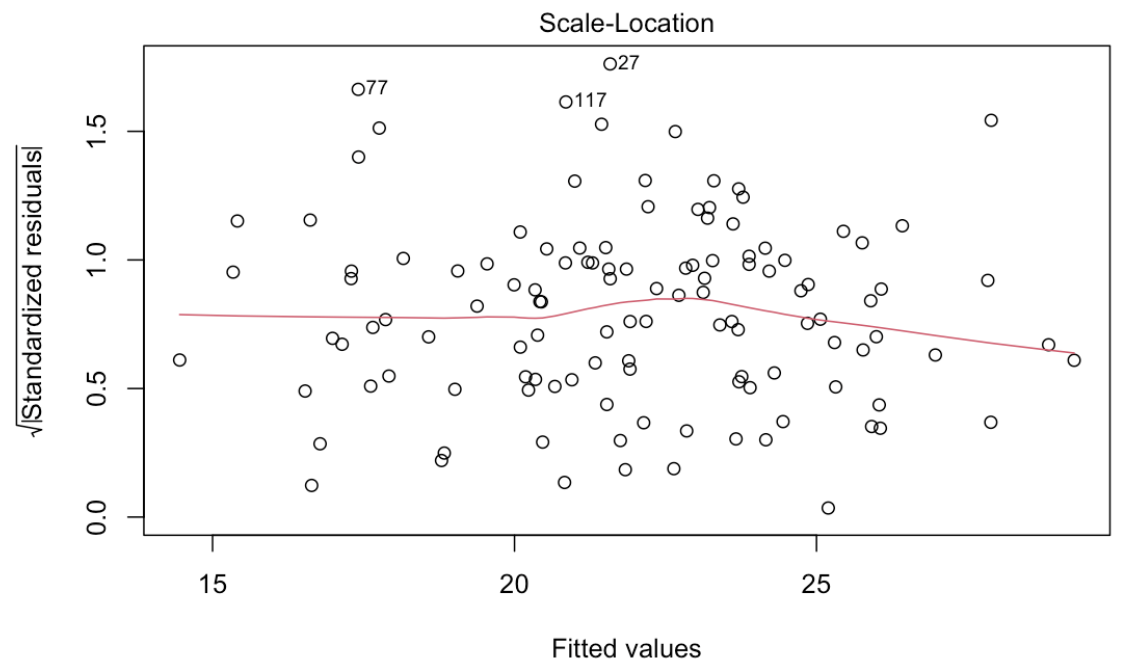
\includegraphics[scale = 0.4]{pics/outlier standardized.png} \label{outlier 27}}

\smallskip

\center{Point 27}

\bigskip

\center{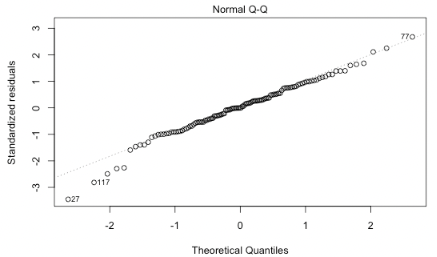
\includegraphics[scale = 0.6]{pics/asine qq.png} \label{asine qq}}

\smallskip

\center{Q-Q plot of arcsine transformation. Point 27 is more extreme in standardized residuals.}

\bigskip

\center{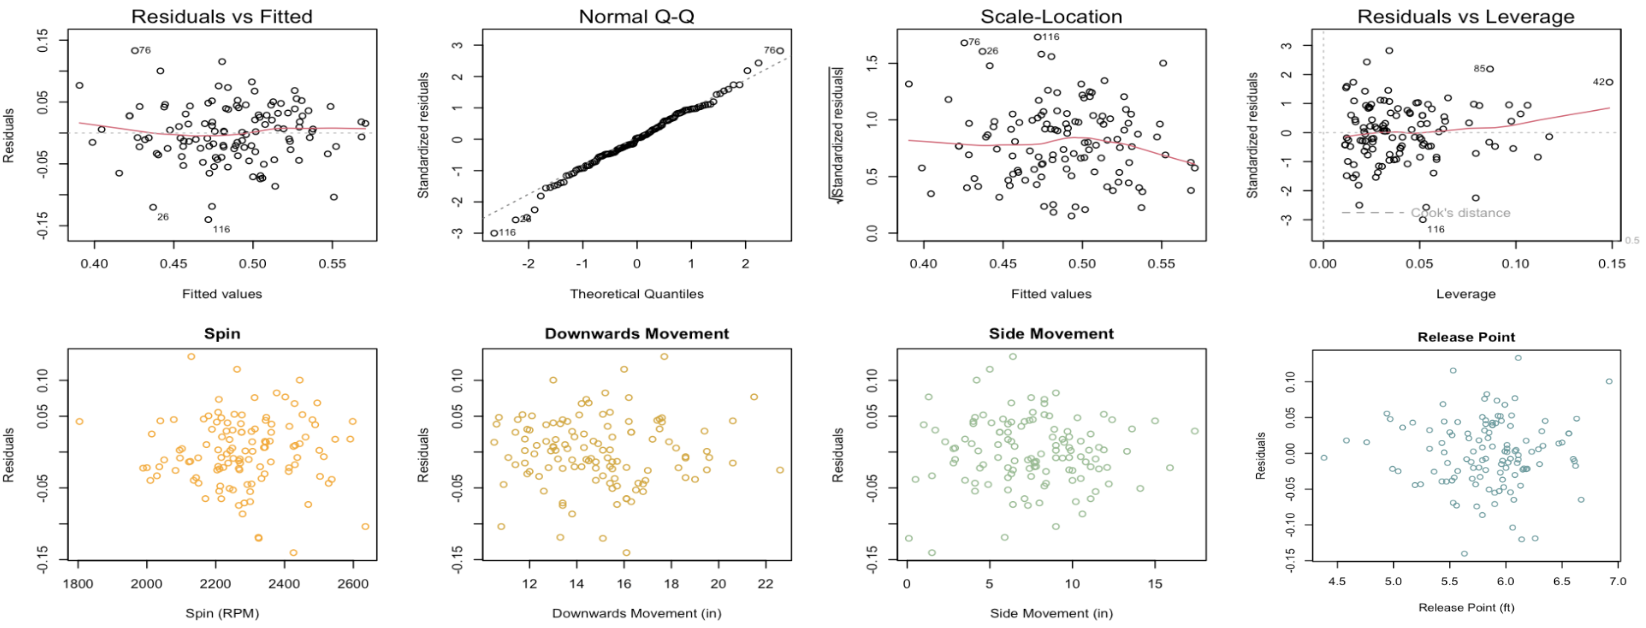
\includegraphics[scale = 0.6]{pics/asine 2.png} \label{asine 2}}

\smallskip

\center{Results of attempting to fix Model 4 via arcsine. Graphs look somewhat worse.}

\newpage


%% Bibliography
\centering{References}

\bigskip

\begin{minipage}{\textwidth}
Bahill, A. T., Baldwin, D. G., \& Venkateswaran, J. (2005). Predicting a Baseball’s Path: A
\end{minipage}


\vspace{0.15 cm}

\hspace*{1cm}
\begin{minipage}{.9\textwidth}
    batter watches the pitcher’s motion plus the spin on the ball to calculate when and where it will cross the plate. \textit{American Scientist}, 93(3), 218–225. http://www.jstor.org/stable/27858576
\end{minipage}

\vspace{0.8 cm}

\begin{minipage}{\textwidth}
Mordkoff, T. (2016). Standard Transformations. \textit{Standard Transformations}. Personal 
\end{minipage}


\vspace{0.15 cm}

\hspace*{1cm}
\begin{minipage}{.9\textwidth}
   Collection of Toby J. Mordkoff, University of Iowa, Iowa City, IA.
\end{minipage}

\vspace{0.8 cm}

\begin{minipage}{\textwidth}
Selin, C.W. (1959). An Analysis of the Aerodynamics of Pitched Baseballs. \textit{Research} 
\end{minipage}

\vspace{0.15 cm}

\hspace*{1cm}
\begin{minipage}{.9\textwidth}
    \textit{Quarterly. American Association for Health, Physical Education and Recreation}, 30, 232-240.
\end{minipage}

\vspace{0.8 cm}

\begin{minipage}{\textwidth}
Sidhu, G., \& Caffo, B. (2014). Moneybarl: Exploiting Pitcher Decision Making Using
\end{minipage}


\vspace{0.15 cm}

\hspace*{1cm}
\begin{minipage}{.9\textwidth}
    Reinforcement Learning. \textit{The Annals of Applied Statistics}, 8(2), 926–955. http://www.jstor.org/stable/24522082
\end{minipage}


\end{document}

\newpage
\setstretch{1}  %reduce bibliography line spacing
\printbibliography
\end{document}